\documentclass[12pt]{article}

\usepackage{amsmath}
\usepackage{amssymb}
\usepackage{amsfonts}
\usepackage{longtable}
\usepackage{array}
\usepackage{graphicx} % Required for inserting images
\usepackage{float} % Allows putting an [H] in \begin{figure} to specify the exact location of the figure
\usepackage[margin=1in]{geometry}
\usepackage[greek, english]{babel}
\usepackage[utf8x]{inputenc}
\usepackage[table]{xcolor}
\usepackage{changepage} % for implementing custom indenting
\usepackage{nopageno}
\usepackage{parskip}
\usepackage{helvet}
\usepackage{hyperref}
\usepackage{url}

% DOCUMENT SETTINGS
\renewcommand\familydefault{\sfdefault} % sans serif
\setlength{\parskip}{0.4cm} % space between paragraphs
\hypersetup{
    colorlinks = true,
    linkcolor = blue,
    filecolor = magenta,      
    urlcolor = blue
}

% COMMAND DEFINITIONS
\newcommand{\myindent}[2]{
    \begin{adjustwidth}{#1}{0pt}
    #2
    \end{adjustwidth}
}
\newcommand{\sectindent}[1]{\myindent{25pt}{#1}}
\newcommand{\subsectindent}[1]{\myindent{30pt}{#1}}

\newcommand{\ro}{\selectlanguage{romanian}}
\newcommand{\gr}{\selectlanguage{greek}}

% DOCUMENT PARAMETERS
\definecolor{mygreen}{RGB}{96, 216, 55}

\title{\vspace{-2em}\textcolor{mygreen}{Image classification using Convolutional Neural Networks on the Imagenette dataset}}
\author{\vspace{-3em}Radu Breazu}
\date{12 November 2024}

\begin{document}

\maketitle

The purpose of this report is to present the results of the image classification task on the Imagenette dataset using Convolutional Neural Networks (CNNs), as well as
to present details about the convolution and filtering operations from the first part of the assignment which have been implemented by hand.

\section{The convolution and filtering operations (Task 1)}
For this task, only the filtering operation has been implemented. The implementation was done, as requested by the assignment, by hand, using just \texttt{numpy}
functions. The implementation is as follows: the shape of the weights matrix and of the input volume are deconstructed, in order to find out all the necessary
information, and then, a volume of $b \times c \times (h - h_{\text{filter}} + 1) \times (w - w_{\text{filter}} + 1)$, where $b$ and $c$ are the batch size and the
number of channels, respectively, is created. This volume is then filled with the dot product of the weights and the input volume, for each input channel and batch. In
order to efficiently implement the matrix operations, the \texttt{torch.dot} and \texttt{torch.sum} functions have been used. The correctness of the implementation
is proven by the following screenshot:

\begin{figure}[H]
    \setlength{\unitlength}{1mm}
    \begin{picture}(0, 0)
        \put(5, -15){
\includegraphics[scale=1]{images/filter_test_passing.png}}
    \end{picture}
    \vspace{1.5cm}
\end{figure}

The photo shows clearly that the last test is passing, given that the last character on the second row is a dot (and not E or F, which indicate either an error -- such
as \\ \texttt{NotImplementedError()} -- or a failure -- a result is computed, but it is not the correct one).

\section{Image classification using handmade CNNs (Task 2)}
For this task, a simple CNN architecture with 3 convolutional layers and 2 fully connected layers has been implemented. The architecture is as follows:
\begin{itemize}
    \item 1 convolutional layer with a kernel size of $3 \times 3$, $16$ filters, a stride size of $1$, a padding of $1$ (in order to preserve the size of the image),
    ReLU activation function and average pooling with a kernel size of $2 \times 2$ and a stride size of $2$
    \item 2 more convolutional layers with a kernel size of $3 \times 3$, $32$ and $64$ filters respectively, a stride size of $1$, ReLU activation function and average
    pooling with a kernel size of $2 \times 2$ and a stride size of $2$. If batch normalization is activated via the corresponding initialization argument, a batch
    normalization layer is added at the end of the convolutional layers
    \item 2 fully connected layers with $128$ and $10$ neurons respectively, ReLU activation function and a dropout layer with a dropout rate of $0.3$ between them (if
    dropout is activated via the corresponding initialization argument)
\end{itemize}

The activation function is ReLU in all cases, since it is an appropriate choice for the hidden layers of a neural network that does multiclass classification (as
opposed to binary classification, case in which the sigmoid or the tanh functions are more appropriate), and it is computationally efficient (unlike softmax). The use
of an activation function is justified by the fact that it increases the learning capabilities of the network, by introducing non-linearities. Furthermore, pooling is
necessary, in order to reduce the dimensions of the input image, as well as preserve relevant information further down the line. During experimentation, average pooling
has produced better results (this may have to do with the fact that it does compress all the information in the area it is applied onto, unlike max pooling, which
chooses just one pixel -- the one with the highest colour values -- and loses the rest of the details), therefore it has been chosen.

The model has been trained using the SGD optimizer, with a learning rate of $7 \cdot 10^{-4}$, a batch size of $16$ and a number of epochs of $30$. The loss function
used is the cross-entropy loss, which is appropriate for multiclass classification tasks. Without any optimizations, the model has achieved an accuracy of $54.75\%$
on the test set. The confusion matrix is presented below.

\begin{figure}[H]
    \setlength{\unitlength}{1mm}
    \begin{picture}(0, 0)
        \put(25, -80){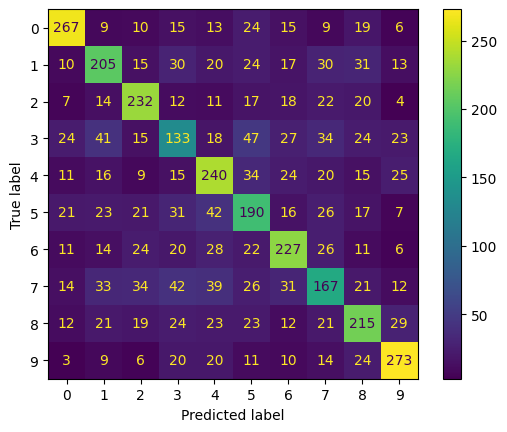
\includegraphics[scale=0.7]{images/confusion_matrix.png}}
    \end{picture}
    \vspace{7cm}
\end{figure}

From the matrix, one can see that the model cannot generalize to a satisfactory degree, as juat under half of all the images are being misclassified. This is most likely due to the
fact that the model has to extract the characteristics of 10 different classes from approximately 350 to 400 images per class, which is not enough to learn the
features of each class (which means that the model is learning the noise in the training set, rather than the features that are actually useful for classification in
general).

Out of all the optimizations, batch normalization has produced the best results, increasing the accuracy to $65.01\%$. Dropout has not produced any significant effect,
since it has managed to increase the accuracy by only $1.65\%$ in the respective test, from $51.21\%$ to $52.86\%$.

\begin{figure}[h]
    \setlength{\unitlength}{1mm}
    \begin{picture}(0, 0)
        \put(20, -75){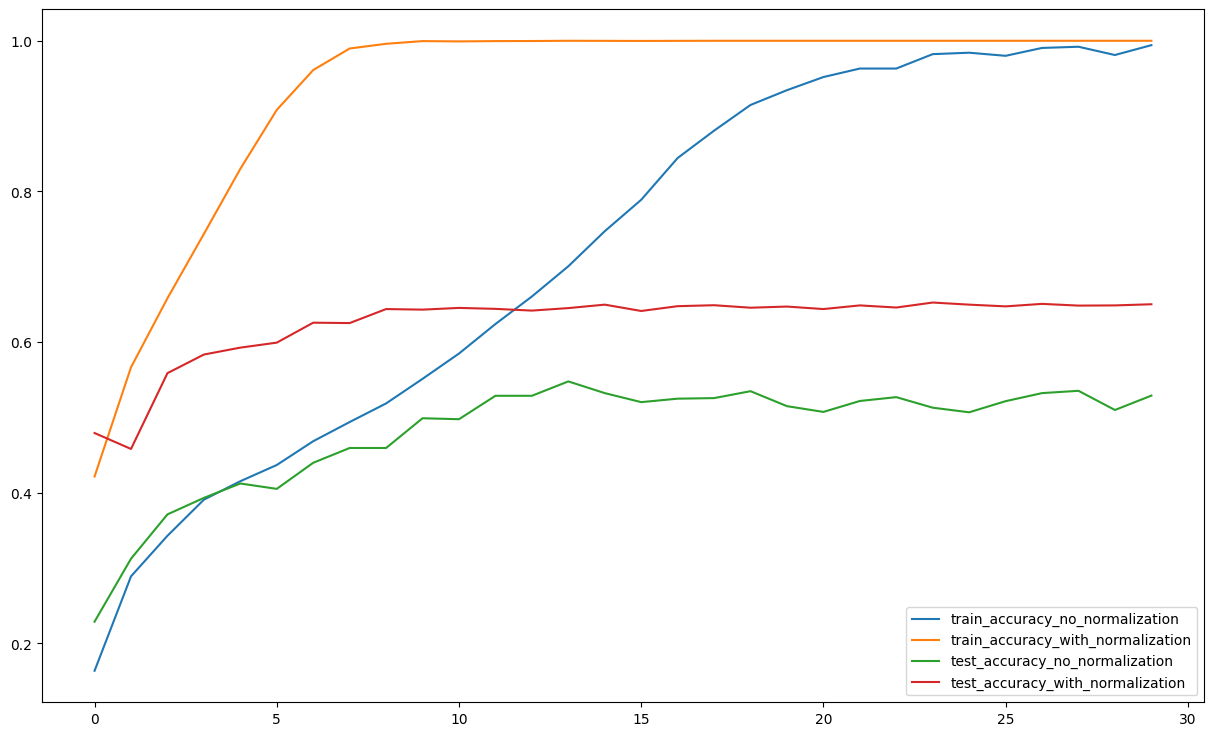
\includegraphics[scale=0.4]{images/accuracy_with_without_normalization.png}}
    \end{picture}
    \vspace{7.5cm}
\end{figure}

\begin{figure}[H]
    \setlength{\unitlength}{1mm}
    \begin{picture}(0, 0)
        \put(20, -75){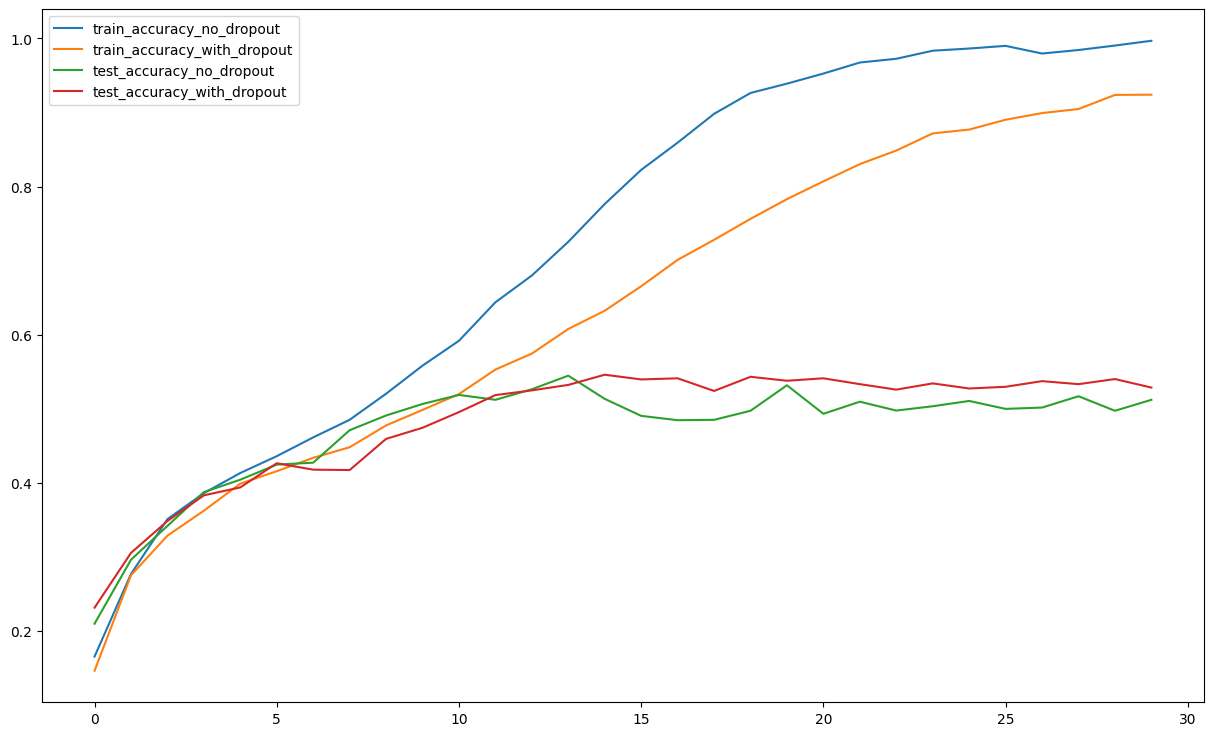
\includegraphics[scale=0.4]{images/accuracy_with_without_dropout.png}}
    \end{picture}
    \vspace{7cm}
\end{figure}

The graphs clearly show that the model is prone to overfitting, since the training accuracy is much higher than the test accuracy. Once again, the most likely reason
is that the model is too complex for the dataset, and it is learning the noise in the training set, rather than the features of the images. Furthermore, it is also
possible that the model might actually not be able to learn the relevant features of the images, due to the small size of the dataset.

\begin{figure}[H]
    \setlength{\unitlength}{1mm}
    \begin{picture}(0, 0)
        \put(5, -95){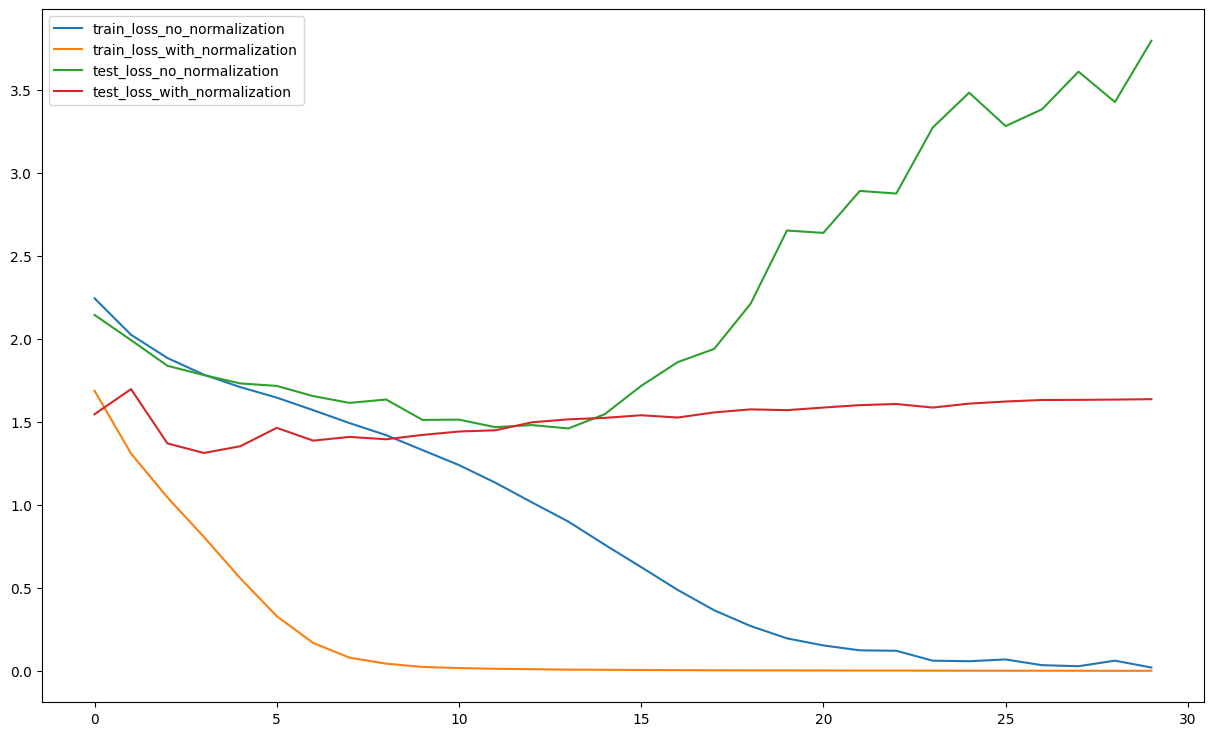
\includegraphics[scale=0.5]{images/loss_with_without_normalization.png}}
    \end{picture}
    \vspace{7cm}
\end{figure}

\begin{figure}[H]
    \setlength{\unitlength}{1mm}
    \begin{picture}(0, 0)
        \put(5, -97){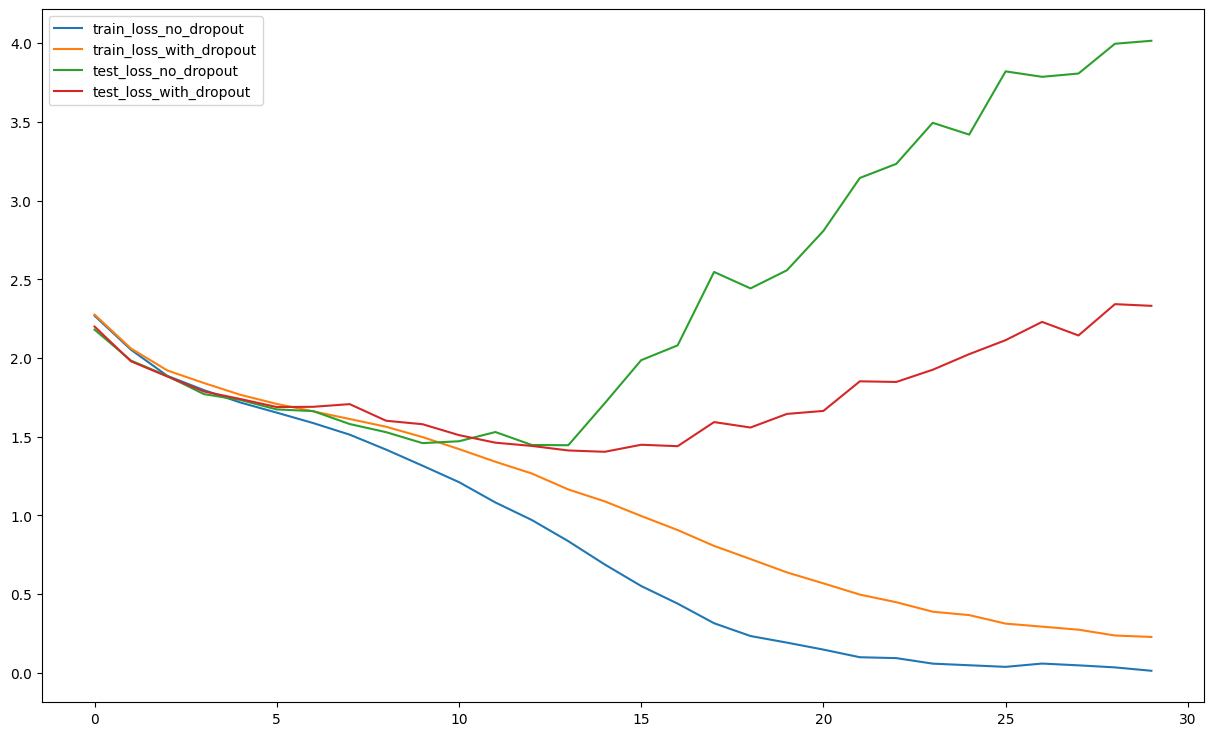
\includegraphics[scale=0.5]{images/loss_with_without_dropout.png}}
    \end{picture}
    \vspace{10cm}
\end{figure}

The last graph shows that the dropout optimization does lead to smaller values of the loss function for the test set. However, the loss does not decrease enough to
make the model learn better the characteristics of the photos, at it is still over $2$.

For the data augmentation part, I have used the following technique: I have made a copy of the original dataset, and I have applied a horizontal flip and a colour
jitter to the images. The horizontal flip was chosen so as to introduce entropy into the new images, and the colour jitter was chosen because it enhances the image
attributes. These transformations have proven to have some efficiency, in that the accuracy of the model increased from $51.28\%$ to $53.40\%$ in the respective test.

\begin{figure}[h]
    \setlength{\unitlength}{1mm}
    \begin{picture}(0, 0)
        \put(5, -97){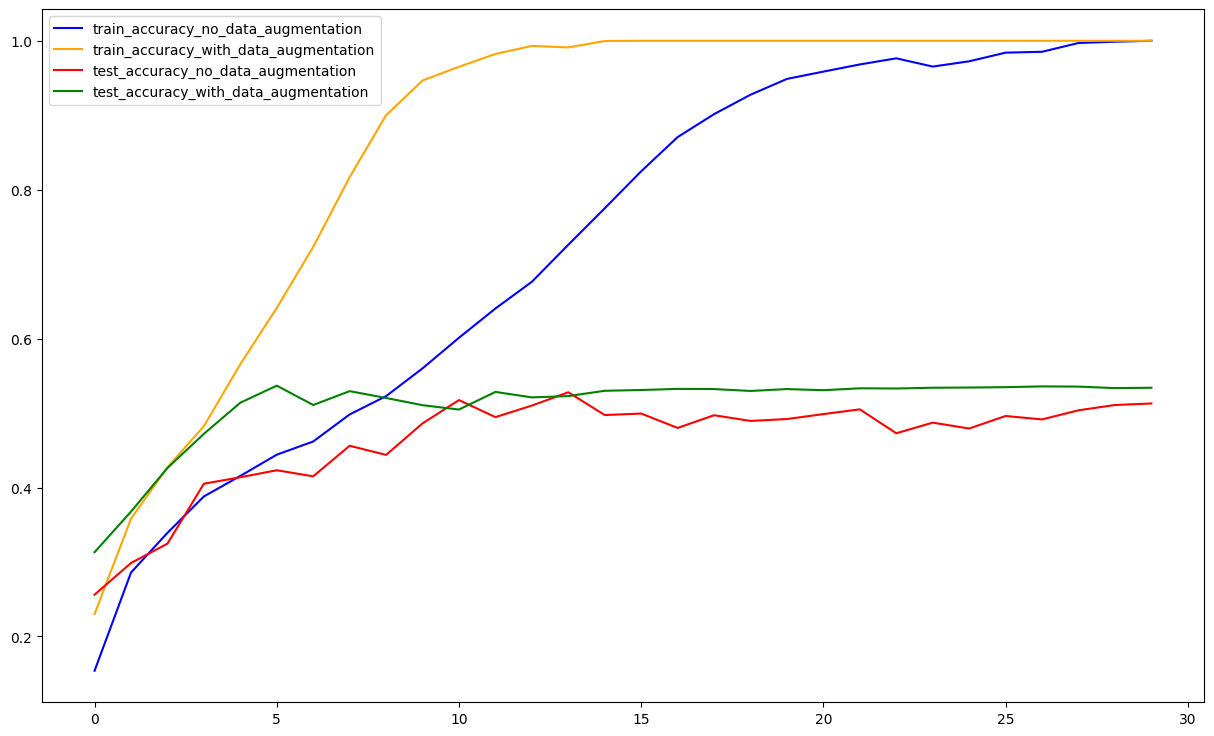
\includegraphics[scale=0.5]{images/accuracy_with_without_data_augmentation.png}}
    \end{picture}
    \vspace{10cm}
\end{figure}

However, surprisingly, the loss function values are higher for the model that uses data augmentation for every epoch after the seventh one, as shown in the graph below.

\begin{figure}[H]
    \setlength{\unitlength}{1mm}
    \begin{picture}(0, 0)
        \put(20, -75){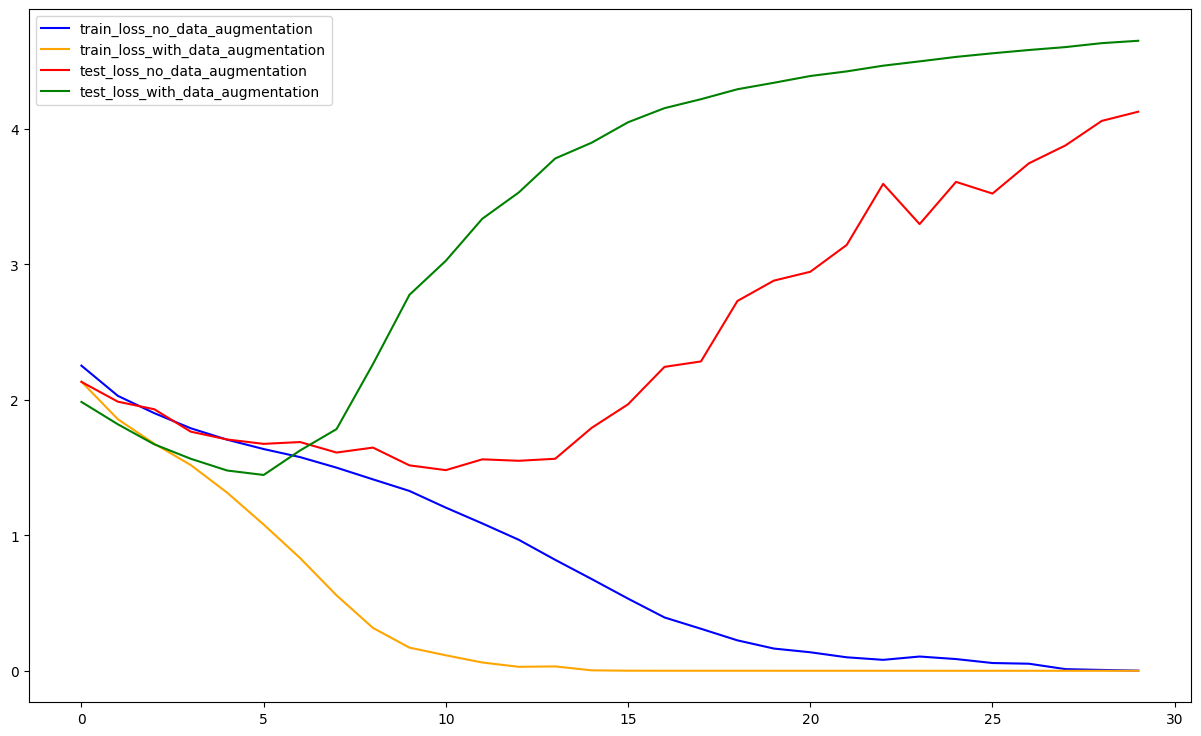
\includegraphics[scale=0.4]{images/loss_with_without_data_augmentation.png}}
    \end{picture}
    \vspace{7cm}
\end{figure}

\section{Image classification using the ResNet architecture (Task 3)}
For this task, the ResNet architecture has been used, with the ResNet-18 variant. This model has successfully classified the images, with an accuracy of $95.08\%$ on
the test set. The confusion matrix is presented below.

\begin{figure}[H]
    \setlength{\unitlength}{1mm}
    \begin{picture}(0, 0)
        \put(25, -97){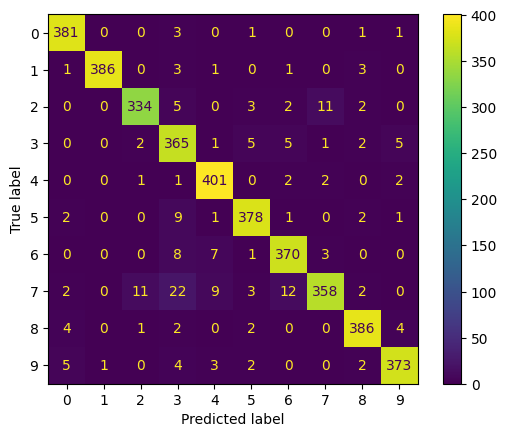
\includegraphics[scale=0.8]{images/confusion_matrix_task_3.png}}
    \end{picture}
    \vspace{10cm}
\end{figure}

The main difference between this model and the simple one, which was implemented in the previous task, is the fact that the ResNet architecture uses residual blocks,
as well as a much higher number of layers overall. Furthermore, the ResNet model was pretrained on the ImageNet dataset, a much bigger dataset than Imagenette, which
has helped it learn the features of the input images. The graphs below show the training and validation loss curves and the accuracy curves.

\begin{figure}[H]
    \setlength{\unitlength}{1mm}
    \begin{picture}(0, 0)
        \put(10, -97){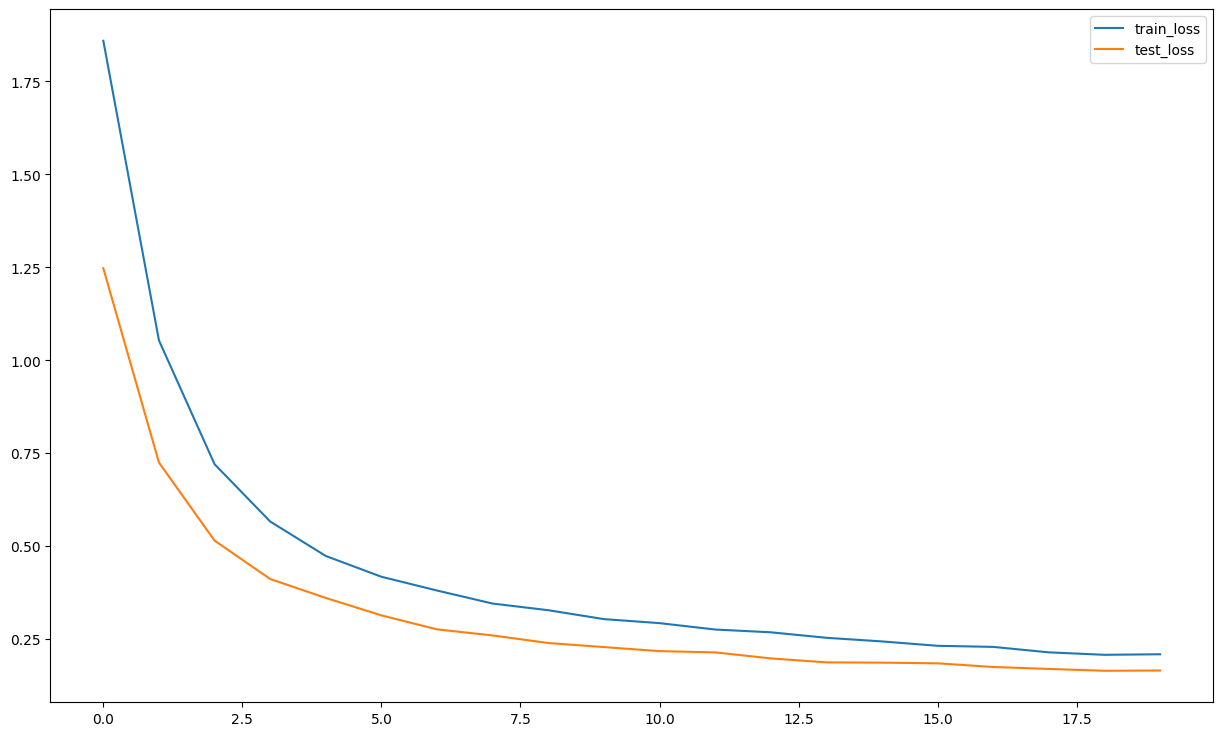
\includegraphics[scale=0.5]{images/train_test_loss_task_3.png}}
    \end{picture}
    \vspace{10cm}
\end{figure}

\begin{figure}[H]
    \setlength{\unitlength}{1mm}
    \begin{picture}(0, 0)
        \put(10, -97){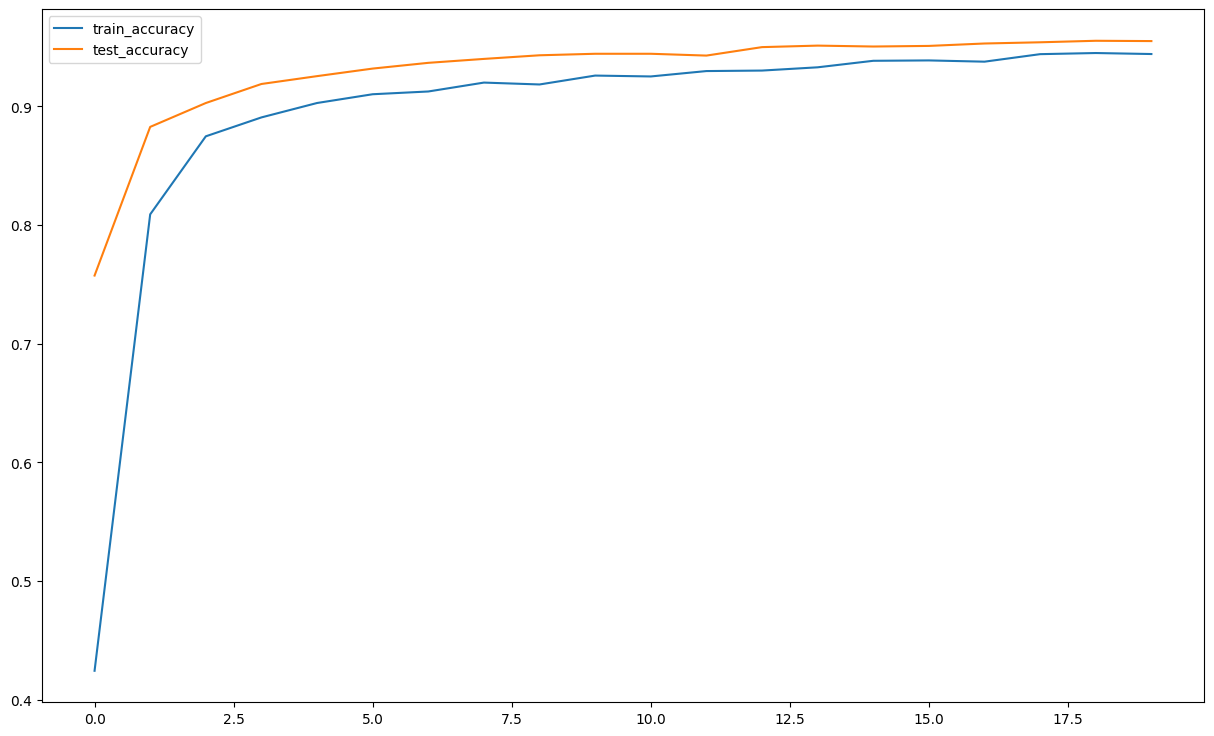
\includegraphics[scale=0.5]{images/train_test_accuracy_task_3.png}}
    \end{picture}
    \vspace{10cm}
\end{figure}

It is evident that the ResNet uses ``prior experience'' from the images it had already been trained on, since for every epoch, the test loss and accuracy are lower
than the training and test loss and accuracy. This means that the model just fine tunes the weights of the pretrained model, in order to classify the images from the
new dataset.

\end{document}